\documentclass[a4paper,hidelinks,14pt]{extarticle}

\usepackage[utf8]{inputenc}
\usepackage[T2A]{fontenc}
\usepackage[english, russian]{babel}
\usepackage{lipsum}
\usepackage{amsmath}
\usepackage{amssymb}
\usepackage{amsfonts}
\usepackage{mathtools}
\usepackage{datetime}
\usepackage[pdftex]{graphicx}
\usepackage{indentfirst}
\usepackage{asymptote}
\usepackage{systeme}
\usepackage[dvipsnames]{xcolor}
\usepackage{lastpage}
\usepackage{fancybox,fancyhdr}
\usepackage{hyperref}
\usepackage[font={small,it}]{caption}
\fancyhead[L]{Лабораторная работа №1}
\fancyhead[C]{}
\fancyhead[R]{Ряды Фурье}
\fancyfoot[L]{}
\fancyfoot[C]{Страница \thepage\space из \pageref{LastPage}}
\fancyfoot[R]{}
\pagestyle{fancy}
\newcommand{\gt}{\textgreater}
\newcommand{\lt}{\textless}

\begin{document}
	\begin{titlepage}
		\setlength{\parindent}{0ex}
		
		\begin{center}
			\textsc{
				\vspace{1ex}
				Научно исследовательский университет ИТМО \\
				\vspace{0.5ex}
				Факультет систем управления и робототехники \\
				\vspace{0.5ex}
			}
		\end{center}
		
		\vspace{50mm}
		
		\begin{center}
			Отчет по лабораторной работе №1 \\
			Ряды Фурье
		\end{center}
		
		\vspace{50mm}
		
		\begin{minipage}{.55\linewidth}
			Выполнил студент группы R3280
			
			Преподаватели
		\end{minipage}
		\hfill
		\begin{minipage}{.5\linewidth}
			\begin{flushright}
				Мовчан И. Е.
				\\
				Пашенко А.В., Перегудин А. А.
			\end{flushright}
		\end{minipage}
		
		\vfill
		\begin{center}
			Санкт-Петербург
			\\
			2024
		\end{center}
		
	\end{titlepage}
	
	\section{Вещественные функции}
	Зададимся положительными числами $a=1$, $b=3$, $t_0=1$, $t_1=2$, $t_2=4$ и рассмотрим вещественные функции $f: \mathbb{R} \rightarrow \mathbb{R}$.
	\subsection{Квадратная волна}
	Имеем $T=t_2-t_0=3$ периодическую фунцию следующего вида:
	\begin{equation*}
	f(t) = \begin{cases}
		a, \ t \in [t_0, t_1), \\
		b, \ \hspace{0.5mm} t \in [t_1, t_2)
	\end{cases}
	\Rightarrow
	f(t) = \begin{cases}
		1, \ t \in [1, 2), \\
		3, \ t \in [2, 4)
	\end{cases}
	\end{equation*}
	
	Рассмотрим частичные суммы $F_N$ и $G_N$ вида
	$$
		F_N = \frac{a_0}{2} + \sum \limits_{n=1}^{N} (a_n \cos(\omega_n t) + b_n \sin(\omega_n t)), \ 
		G_N = \sum \limits_{n=-N}^{N} c_n e^{i \omega_n t}
	$$
	
	Коэффициенты разложения вычисляются по формулам:
	$$
	a_n = \frac{2}{T} \int \limits_{1}^{4}f(t)\cos\left(\frac{2\pi n}{T} t\right) dt, \ 
	b_n = \frac{2}{T} \int \limits_{1}^{4}f(t)\sin\left(\frac{2\pi n}{T} t\right) dt, n \geq 0
	$$
	
	Откуда 
	$$
	a_n = \frac{2}{3} \int \limits_{1}^{4}f(t)\cos\left(\frac{2\pi n}{3} t\right) dt, \ 
	b_n = \frac{2}{3} \int \limits_{1}^{4}f(t)\sin\left(\frac{2\pi n}{3} t\right) dt, n \geq 0
	$$
	
	А 
	$$
	c_n = \frac{1}{T} \int \limits_{1}^{4} f(t) e^{-i \omega_n t} dt = \frac{1}{3} \int \limits_{1}^{4} f(t) e^{-i \omega_n t} dt,
	$$
	$$
	\text{где }\omega_n = \frac{2 \pi n}{T} = \frac{2\pi n}{3}
	$$
	
	Нахождение коэффициентов сводится к следующим операциям:
	$$
	a_n = \frac{2}{3} \int\limits_{1}^{2} \cos\left(\frac{2\pi n}{3} t\right) dt + \frac{2}{3} \int\limits_{2}^{4} 3 \cos\left(\frac{2\pi n}{3} t\right) dt =
	$$
	$$
	= \frac{2}{3} \int\limits_{1}^{2} \cos\left(\frac{2\pi n}{3} t\right) dt + 2 \int\limits_{2}^{4} \cos\left(\frac{2\pi n}{3} t\right) dt =
	$$
	$$
	=\frac{\sin\left(\frac{4 \pi n}{3} \right) - \sin\left(\frac{2 \pi n}{3} \right)}{\pi n} + 3\frac{\sin\left(\frac{8 \pi n}{3} \right) - \sin\left(\frac{4 \pi n}{3} \right)}{\pi n} =
	$$
	$$
	=\frac{3\sin\left( \frac{8\pi n}{3} \right) -2\sin\left(\frac{4 \pi n}{3} \right) - \sin\left(\frac{2 \pi n}{3} \right)}{\pi n},
	$$
	
	$$
	a_0 = \frac{2}{3} \int\limits^{2}_{1} dt + 2 \int\limits^{4}_{2} dt = \frac{2}{3} + 4 = \frac{14}{3},\ b_0 = 0
	$$
	
	$$
	b_n =\frac{2}{3} \int\limits_{1}^{2} \sin\left(\frac{2\pi n}{3} t\right) dt + 2 \int\limits_{2}^{4} \sin\left(\frac{2\pi n}{3} t\right) dt =
	$$
	$$
	= -\frac{\cos\left(\frac{4 \pi n}{3} \right) - \cos\left(\frac{2 \pi n}{3} \right)}{\pi n} - 3\frac{\cos\left(\frac{8 \pi n}{3} \right) - \cos\left(\frac{4 \pi n}{3} \right)}{\pi n} =
	$$
	$$
	=-\frac{3\cos\left( \frac{8\pi n}{3} \right) -2\cos\left(\frac{4 \pi n}{3} \right) - \cos\left(\frac{2 \pi n}{3} \right)}{\pi n},
	$$
	
	$$
	c_n = \frac{1}{3} \int\limits_{1}^{2} e^{-i\omega_n t} dt + \int\limits_{2}^{4} e^{-i\omega_n t} dt = \frac{i(e^{-2i\omega_n} - e^{-i\omega_n})}{3\omega_n} + \frac{i(e^{-4i\omega_n} - e^{-2i\omega_n})}{\omega_n}.
	$$
	
	Для $n=1,2$ и вещественного случая:
	$$
	a_1 = \frac{3\sin\left( \frac{8\pi}{3} \right) -2\sin\left(\frac{4 \pi}{3} \right) - \sin\left(\frac{2 \pi}{3} \right)}{\pi},\ 
	a_2 = \frac{3\sin\left( \frac{16\pi}{3} \right) -2\sin\left(\frac{8 \pi}{3} \right) - \sin\left(\frac{4\pi}{3} \right)}{2\pi} 
	$$
	
	Откуда
	
	$$
	a_1 = \frac{\frac{3\sqrt{3}}{2} + \sqrt{3} + \frac{\sqrt{3}}{2}}{\pi} = \frac{3\sqrt{3}}{\pi},\ a_2 = -\frac{2\sqrt{3}}{2\pi}=-\frac{\sqrt{3}}{\pi}.
	$$
	
	Для косинусов имеем: 
	$$
	b_1 = -\frac{3\cos\left( \frac{8\pi}{3} \right) -2\cos\left(\frac{4 \pi}{3} \right) - \cos\left(\frac{2 \pi}{3} \right)}{\pi} = 0,\  b_2 = 0	
	$$
	
	Рассмотрим графики:
	\begin{figure}[h]
		\centering
		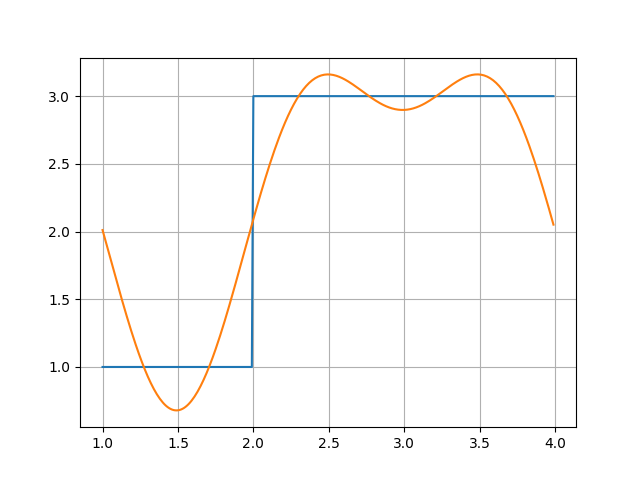
\includegraphics[scale=0.65]{images/k=2.png}
		\caption{Графики для значений коэффициентов $(a_n, b_n)$ для $k=2$}
	\end{figure}
	
	\begin{figure}[h]
		\centering
		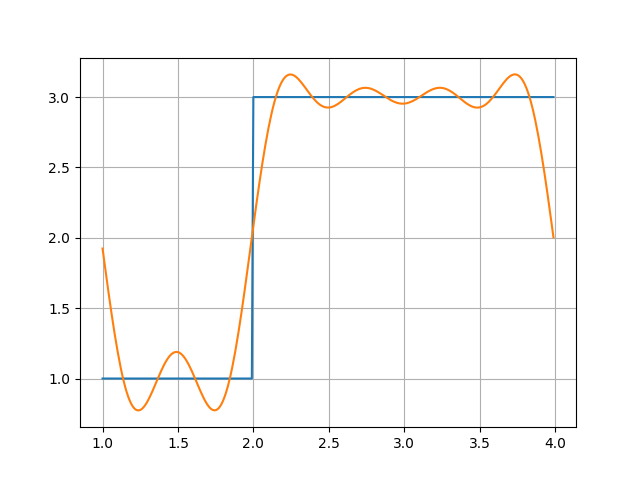
\includegraphics[scale=0.65]{images/k=5.png}
		\caption{Графики для значений коэффициентов $(a_n, b_n)$ для $k=5$}
	\end{figure}
	
	\begin{figure}[h]
		\centering
		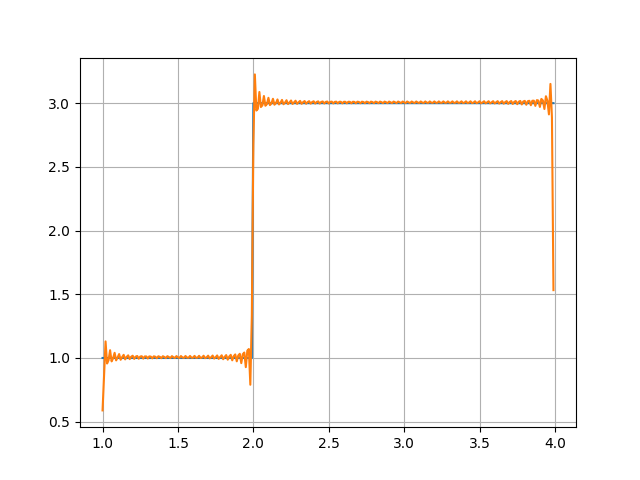
\includegraphics[scale=0.65]{images/k=100.png}
		\caption{Графики для значений коэффициентов $(a_n, b_n)$ для $k=100$}
	\end{figure}
	
	
	
\end{document}